%%%%%%%%%%%%%%%%%%%%%%%%%%%%%%%%%%%%%%%%%%%%%%%%%%%%%%%%%%%%%%%%%%%%%%%%%%%%%%%%
%% BEFORE YOU START:
%%
%% 1. Rename the paper.tex file into your paper name. Use the BibTeX key policy
%%    for the naming convention (see end of this file)
%%
%% 2. Change line 3 in the Makefile from "TARGET=paper" to "TARGET=name-of-tex-file"
%%
%%%%%%%%%%%%%%%%%%%%%%%%%%%%%%%%%%%%%%%%%%%%%%%%%%%%%%%%%%%%%%%%%%%%%%%%%%%%%%%%

\documentclass[letterpaper, 10 pt, conference]{ieeeconf}
\IEEEoverridecommandlockouts    % This command is only needed if
\overrideIEEEmargins            % Needed to meet printer requirements.

\input{stachnisslab-latex}
\input{stachnisslab-math}
\usepackage{multirow}
\usepackage[table]{xcolor}

\usepackage{fontspec}   % XeLaTeX 字体设置
\usepackage{xeCJK}      % 中文支持
\setCJKmainfont{SimSun} % 中文主字体(宋体)
\setCJKsansfont{SimHei} % 中文无衬线字体(黑体)
\setCJKmonofont{FangSong} % 中文等宽字体(仿宋)
\usepackage{orcidlink}


%% Aligns the last page but causes errors on 
%% some machines (such as OSX), so don't use it for now.
% \usepackage{flushend}

%% Style hacks to save space between floating objects and text
%\setlength{\textfloatsep}{1.3em}
%\setlength{\dbltextfloatsep}{1.3em} 
\makeatletter
\def\blfootnote{\gdef\@thefnmark{}\@footnotetext}
\makeatother

\newcommand{\datasetName}[0]{TODO\xspace} %% macro for printing the dataset name.

%%%%%%%%%%%%%%%%%%%%%%%%%%%%%%%%%%%%%%%%%%%%%%%%%%%%%%%%%%%%%%%%%%%%%%%%%%%%%%%%
%% 中文翻译版本 - 保持原有LaTeX结构
\title{\LARGE \bf 真实果园环境中跨不同传感器的\\3D层次化全景分割}

\author{Matteo Sodano \qquad Federico Magistri \qquad Elias Marks \qquad Fares Hosn \qquad Aibek Zurbayev \\ Rodrigo Marcuzzi \qquad Meher V. R. Malladi \qquad Jens Behley \qquad Cyrill Stachniss% <-this % stops a space
  \thanks{All authors are with the Center for Robotics, University of Bonn, Germany. Cyrill Stachniss is additionally with the Department of Engineering Science at the University of Oxford, UK, and with the Lamarr Institute for Machine Learning and Artificial Intelligence, Germany.}%
  \thanks{This work has partially been funded 
  by the Deutsche Forschungsgemeinschaft (DFG, German Research Foundation) under Germany's Excellence Strategy, EXC-2070 -- 390732324 -- PhenoRob and under STA~1051/5-1 within the FOR 5351~(AID4Crops),
  by the European Union's Horizon Europe research and innovation programme under grant agreement No~101070405~(DigiForest),
  and by the BMBF in the project ``Robotics Institute Germany'', grant No.~16ME0999.
  }%
}

\begin{document}

\twocolumn[{%
\renewcommand\twocolumn[1][]{#1}% 

\maketitle
\thispagestyle{empty}
\pagestyle{empty}

\begin{center}
    \centering
    \vspace{-1.5em}
    \captionsetup{type=figure}
    \includegraphics[width=.92\linewidth]{pics/motivation.pdf}
    % \vspace{.5em}
    \captionof{figure}{使用地面激光扫描仪(TLS)记录的苹果园视图(顶行),用于训练我们的层次化全景分割网络。测试集由对应不同传感器和机器人的不同子集组成。图中所示的两个示例分别是配备PhaseOne iXM-100相机的无人机(UAV)和配备RealSense d435i相机的地面机器人(UGV)。}
    \label{fig:motivation}
\end{center}%
}]

% \makeatletter{\renewcommand*{\@makefnmark}{}
% \footnotetext{All authors are with the Center for Robotics, University of Bonn, Germany. Cyrill Stachniss is additionally with the Department of Engineering Science at the University of Oxford, UK, and with the Lamarr Institute for Machine Learning and Artificial Intelligence, Germany.}\makeatother
% \footnotetext{This work has partially been funded 
%   by the Deutsche Forschungsgemeinschaft (DFG, German Research Foundation) under Germany's Excellence Strategy, EXC-2070 -- 390732324 -- PhenoRob,
%   by the Deutsche Forschungsgemeinschaft (DFG, German Research Foundation) under \mbox{STA~1051/5-1} within the FOR 5351~(AID4Crops),
%   % by the European Union’s Horizon 2020 research and innovation programme under grant agreement No~101017008~(Harmony), 
%   by the European Union's Horizon Europe research and innovation programme under grant agreement No~101070405~(DigiForest).
%   }
%   % and 
%   % by the Federal Ministry of Food and Agriculture~(BMEL) based on a decision of the Parliament of the Federal Republic of Germany via the Federal Office for Agriculture and Food~(BLE) under the innovation support programme under funding no~28DK108B20~(RegisTer).}\makeatother
% }

% and 
% by the Federal Ministry of Food and Agriculture~(BMEL) based on a decision of the Parliament of the Federal Republic of Germany via the Federal Office for Agriculture and Food~(BLE) under the innovation support programme under funding no~28DK108B20~(RegisTer).}\makeatother

\thispagestyle{empty}
\pagestyle{empty}
% \maketitle


%%%%%%%%%%%%%%%%%%%%%%%%%%%%%%%%%%%%%%%%%%%%%%%%%%%%%%%%%%%%%%%%%%%%%%%%%%%%%%%%
\begin{abstract}
  作物产量估计是农业中的一个重要问题,因为准确的产量估计可以支持农民在收获或精准干预方面的决策。机器人可以帮助实现这一过程的自动化。为此,它们需要能够感知周围环境,以识别目标对象,如树木和植物。在本文中,我们提出了一种新方法,用于解决来自不同传感器的3D数据上苹果园的层次化全景分割问题。我们的方法能够同时提供语义分割、树干和果实的实例分割,以及树木的实例分割(一个树干及其果实)。这使我们能够识别相关信息,如单个植物、果实和树干,并捕获它们之间的关系,例如精确估计果园中每棵树关联的果实数量。
  为了有效评估我们的层次化全景分割方法,我们提供了一个专门为此任务设计的数据集。我们的数据集在德国波恩的真实苹果园中采集,使用了多种传感器,从地面激光扫描仪到安装在不同机器人平台上的RGB-D相机。
  实验表明,我们的方法在农业领域的3D全景分割方面超越了现有最先进的方法,同时还提供了完整的层次化全景分割。我们的数据集可在 \mbox{\url{https://www.ipb.uni-bonn.de/data/hops/}} 公开获取。我们方法的开源实现可在 \url{https://github.com/PRBonn/hapt3D} 获取。
  %% 如何与什么
  % 大约3句话解释如何一般性地解决问题并回答:
  % 如何一般性地解决问题?(1/2 - 1句话)
  % 我们的方法有什么特别之处?我们实际在做什么?有什么新内容?
  
  %% 实现、评估、后续
  % 1-2句话说明实验展示了什么,以及你的出色工作对研究社区或世界其他地方的潜在影响 ;-)
\end{abstract}


\blfootnote{所有作者均来自德国波恩大学机器人中心。Cyrill Stachniss同时任职于德国拉马尔机器学习与人工智能研究所。

本工作部分资助来源:德国联邦教育与研究部(BMBF)``德国机器人研究所''项目,资助编号~\mbox{16ME0999};德国研究基金会(DFG)卓越战略项目EXC-2070 -- 390732324 -- PhenoRob,以及FOR 5351~(AID4Crops)项目下的\mbox{STA~1051/5-1};欧盟地平线欧洲研究与创新计划资助协议No~101070405~(DigiForest)。}

%%%%%%%%%%%%%%%%%%%%%%%%%%%%%%%%%%%%%%%%%%%%%%%%%%%%%%%%%%%%%%%%%%%%%%%%%%%%%%%%
\section{引言}
\label{sec:intro}

%%%%%%%%%%%%%%%%%%%
%% 为什么: 
% 首先回答为什么的问题:为什么这很重要?为什么我应该有动力阅读这篇论文?
% 为什么我应该关心?(1段,2-5句话)
作物产量估计是农业中的一项重要任务。准确的产量估计可以帮助农民做出管理决策,以提高作物产量并优化关键因素,如收获时间和施肥用量~\cite{li2018plants, vanklompenburg2020cea, xu2019ei},以及实现精准干预~\cite{blok2025cea}。
机器人可以自动化或支持许多这些干预措施,但要可靠和稳健地做到这一点,它们需要通过解释传感器数据来理解周围环境。
在园艺中,分割、计数和定位果园中的果实等任务至关重要,因为它们是替代人工采果所必需的,而人工采果是一个极其劳动密集型的过程~\cite{calvin2010book}。 

%%%%%%%%%%%%%%%%%%%
%% 解决什么问题
% 其次,解释你正在解决/处理哪个问题。
最近,许多方法针对农业中的感知任务。语义分割~\cite{lottes2019jfr, milioto2018icra}和全景分割~\cite{marks2023ral, roggiolani2022icra, weyler2022ral}尤为常见。这也推动了农业感知任务数据集的发布~\cite{hani2020ral, kierdorf2022jfr, weyler2024pami}。然而,真实农业环境的3D数据集并不常见~\cite{dutagaci2020pm, schunck2021po}。

% In this paper, we propose an approach and a dataset for 3D hierarchical panoptic segmentation in real apple orchards. 
% We recorded data of the apple orchard at different growth stages with different sensors across several crop rows in the span of two years, and labeled the resulting point clouds in order to obtain semantic segmentation, tree instance segmentation, as well as fruit and trunk instance segmentation. Specifically, in the tree instance segmentation each trunk has a label that is shared with all fruits belonging to it. The fruit and trunk instance segmentation yields a different instance for each individual trunk and fruit. Additionally, we propose the first method to address this multi-stage segmentation tasks, while also exploiting the underlying hierarchical relationship between the tasks~\cite{roggiolani2022icra}. We show a portion of the dataset and an exemplary image of the approach we propose in~\figref{fig:motivation}.

本文的主要贡献是双重的。首先,我们提出了一种基于卷积神经网络(CNN)的层次化全景分割方法,该方法能够同时处理多个实例分割任务,同时通过新颖的跳跃连接方案利用它们之间的底层层次关系。其次,我们引入了一个名为HOPS(层次化果园全景分割,hierarchical orchard panoptic segmentation)的真实苹果园3D点云数据集,使用各种传感器录制,如地面激光扫描仪、RGB-D相机或RGB相机配合后续的光束法平差。此外,我们发布了用于层次化全景分割的高质量标注。我们在两年内跨多个作物行的不同生长阶段录制了苹果园的数据,并标记了生成的点云以获得语义分割、树木实例分割以及果实和树干实例分割。具体来说,在树木实例分割中,每个树干都有一个与属于它的所有果实共享的标签。因此,在这个实例级任务中,果实不是单独标记的。果实和树干实例分割为每个单独的树干和果实产生不同的实例。我们在图~\figref{fig:motivation}中展示了数据集的一部分和我们提出的方法的示例图像。


%%%%%%%%%%%%%%%%%%%
%% 我们的核心声明(可以与上述主要贡献合并)
% 明确地陈述你的声明,并确保在实验中再次提及并支持每个声明。

我们的实验表明:%
(i) 我们的方法可以在使用不同传感器获取的真实世界3D数据上联合执行语义分割、树木实例分割和标准实例分割;
%
以及
(ii) 我们的跳跃连接方案使 CNN 能够利用各个分割任务之间的底层层次关系,从而获得更好的分割性能。
%
我们的声明得到了本文和实验评估的支持。 

%%%%%%%%%%%%%%%%%%%%%%%%%%%%%%%%%%%%%%%%%%%%%%%%%%%%%%%%%%%%%%%%%%%%%%%%%%%%%%%%
\section{相关工作}
\label{sec:related}

% 讨论主要相关工作并引用关键论文。
% 相关工作部分应该约为1栏长。
% 可以分段组织,将论文分组,用1-2句话描述关键方法。
% 避免单调的论文枚举。

语义场景解释通常是实现农业机器人自动化所必需的,因为它识别场景中与任务相关的对象,从而实现监测~\cite{lottes2018iros, pan2023iros,smitt2024ral-pagn}和干预~\cite{magistri2024ral,arad2020jfr,lehnert2020jfr}等应用。

%% 3D点云的全景分割
全景分割~\cite{kirillov2019cvpr-ps}统一了语义分割和实例分割,同时提供背景类(所谓的``stuff'')的语义和前景对象(所谓的``things'')的对象级实例。
虽然图像通常用于农业领域的全景分割~\cite{weyler2022ral},但由\mbox{RGB-D}相机、LiDAR或摄影测量运动恢复结构方法生成的3D点云由于能够提取高精度果实抓取~\cite{magistri2024ral,lehnert2020jfr}、植物分割~\cite{montes2020iros}和细粒度性状估计~\cite{marks2023ral}所需的精确几何信息而受到越来越多的研究关注~\cite{zhu2024scidata}。
3D全景分割在自动驾驶领域得到了积极研究~\cite{sirohi2021tro,milioto2020iros,zhou2021cvpr-pplp},其中大多数方法使用共享编码器的特征为语义分割和实例分割使用专用分支。
对于植物表型分析,我们可以利用植物的层次结构,将其分解为单独的部分~\cite{gueldenring2024ral},如植物、叶子甚至更细粒度的叶子结构。这种层次结构已在文献中被利用,利用解码器之间的跳跃连接进行基于图像的层次化自下而上实例预测任务~\cite{roggiolani2022icra},这是我们3D全景分割方法的基础。

与先前的3D全景分割方法相比,我们还通过新颖的跳跃连接方案明确考虑了预测任务的层次结构,这使我们能够预测由植物实例和果实实例组成的层次化语义场景解释,可用于农业领域的植物监测和产量估计。虽然我们的方法应用于果园场景,但层次化全景分割框架是通用的,可以应用于其他领域,如身体部位分割~\cite{lin2020tcsvt}。

%% 数据集
虽然大多数用于语义解释的农业数据集仅提供RGB图像~\cite{lu2020compag},但最近3D数据集已经可用。
特别是,BUP20~\cite{smitt2024ral-pagn}提供了一个用于温室中甜椒实例分割的RGB-D数据集~\cite{smitt2021icra}。
对于真实农业田地中的3D植物表型分析,BonnBeetClouds~\cite{marks2024iros}提供了由甜菜植物的植物和叶子实例组成的标注运动恢复结构点云。
其他数据集使用高精度LiDAR扫描仪~\cite{schunck2021po}或X射线成像~\cite{dutagaci2020pm}在实验室中获取的点云提供植物的器官级标注。
Crops3D数据集~\cite{zhu2024scidata}为使用地面激光扫描仪(TLS)在田间获取的点云数据和使用RGB图像的运动恢复结构或使用结构光相机的单株植物点云提供了不同作物品种的器官级标注。

%% 简要总结自身贡献
与现有的用于语义场景解释的农业数据集相比,我们提供了一个特定领域的果园农业数据集,使用不同传感器录制,并标注了植物和果实实例。
我们提供了使用TLS录制的高分辨率点云,以及使用配备高分辨率RGB相机或机器人中常用的消费级RGB-D传感器的机器人平台获取的运动恢复结构点云数据。



\begin{figure*}
    \centering
    \includegraphics[width=.9\linewidth]{pics/architecture.pdf}
    \caption{编码器将带颜色的点云作为输入,生成的特征由解码器处理。我们在编码器和解码器的每个下采样和上采样块之后使用层次化跳跃连接。我们使用HDBSCAN获取实例。}
    \label{fig:architecture}
    \vspace{-1em}
\end{figure*}

%%%%%%%%%%%%%%%%%%%%%%%%%%%%%%%%%%%%%%%%%%%%%%%%%%%%%%%%%%%%%%%%%%%%%%%%%%%%%%%%
\section{我们的层次化全景分割方法}
\label{sec:main}
我们提出了一种层次化全景分割方法,即同时执行语义分割和具有底层层次关系的多个实例分割任务。我们使用的网络是编码器-解码器架构,解码器处理语义分割和两级实例分割,如图~\figref{fig:architecture}所示。第一个实例分割旨在识别``树木''实例,其中一棵树由一个树干和属于它的所有果实定义。第二个实例分割寻找点云中的所有单独实例(即树干和果实)。

\subsection{网络架构}
我们使用基于MinkUNet的神经网络~\cite{choy2019cvpr}来实现我们的方法。这类神经网络受到UNet~\cite{ronneberger2015micc}设计的启发,其中编码器和解码器通过跳跃连接连接。为了处理3D数据,MinkUNet网络使用稀疏3D卷积来处理输入数据。具体来说,我们使用MinkUNet14A模型,这使我们能够拥有一个轻量级网络。事实上,MinkUNet14A是标准MinkUNet14模型的修改版本,每层具有更少的特征通道,允许更快的计算。我们保持网络的原始结构,并将原始解码器额外复制两次。这使我们能够拥有三个相同的解码器来处理我们旨在解决的三个分割任务,这是利用它们之间底层层次结构的便捷解决方案。

\begin{figure*}
    \centering
    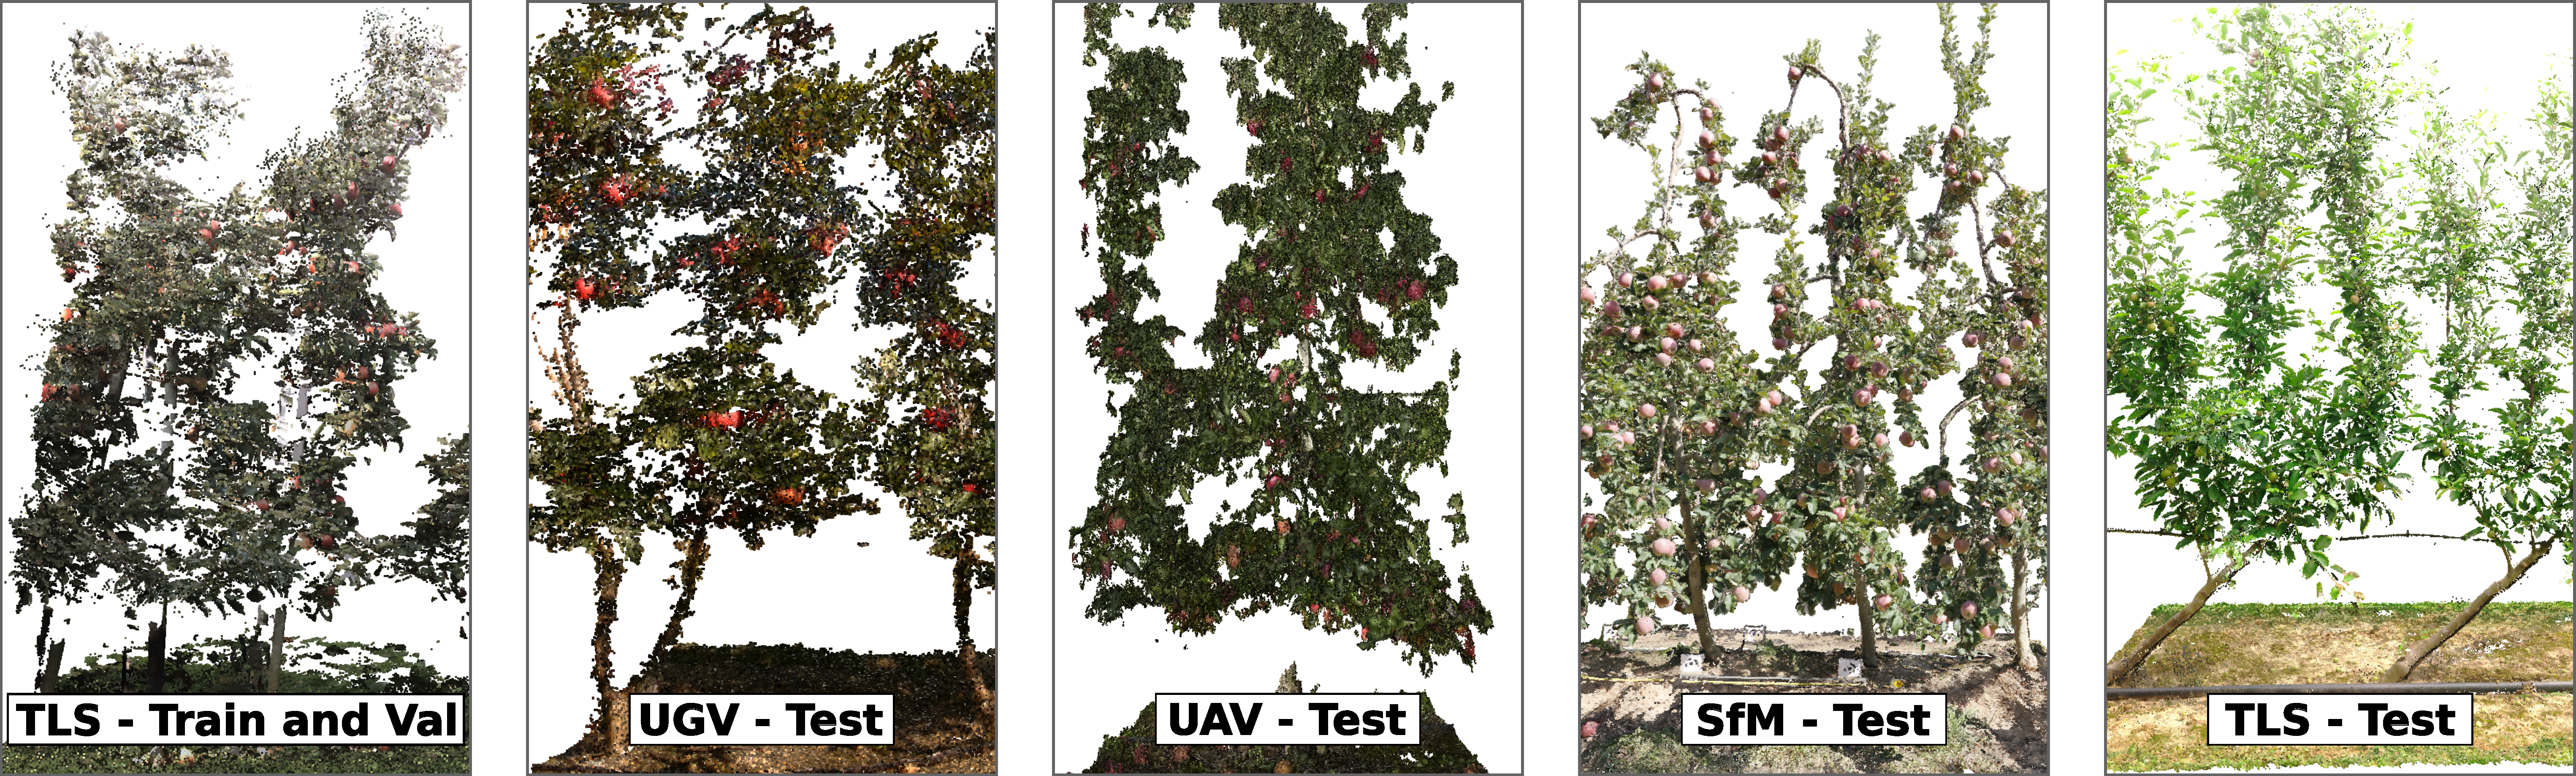
\includegraphics[width=.9\linewidth]{pics/dataset.pdf}
    \caption{HOPS带颜色点云的示例。训练集和验证集的点云使用TLS获取。我们有四个使用不同传感器录制的测试集。名为``SfM''的测试集包含来自Fuji-SfM数据集~\cite{genemola2020compag,genemola2020db}的点云。}
    \label{fig:data}
    \vspace{-1.5em}
\end{figure*}

第一个解码器针对\textit{语义分割},具有深度等于数据集中出现的语义类别数量的单个输出头。它使用标准加权交叉熵损失进行优化:
\begin{equation}
  \mathcal{L}_{\mathrm{sem}} = - \frac{1}{|\mathcal{S}|} \sum_{\b{p} \in \mathcal{S}} \omega_k \, \b{t}_{p}^\top \, \log(\sigma(\b{f}_p)),
\end{equation}
其中 $|\mathcal{S}|$ 是点云中的点数,$\b{p}$ 表示单个点,$\omega_k$ 是通过数据集中每个类别的逆频率计算的类别权重,其中 $k \in \{1, \, \dots, \, K\}$ 表示语义类别,$\b{t}_p \in \mathbb{R}^{K}$ 是点位置 $\b{p}$ 处的独热编码真值标注,$\sigma(\cdot)$ 表示softmax操作,$\b{f}_p$ 表示在点 $\b{p}$ 处预测的softmax前特征。   

第二个解码器针对\textit{树木实例分割},即找到树木实例的任务,其中一棵树定义为一个树干和属于它的所有苹果。这个解码器也有一个用于偏移预测的单个输出头。因此,每个点预测一个指向3D空间中某个位置的3D位移,以便通过聚类促进实例分离。我们为每个点 $\b{p}$ 预测一个偏移 $\b{o}_p \in \mathbb{R}^3$,使得 $\b{e}_p = \b{p} + \b{o}_p$ 是点被位移到的3D位置。为了使属于同一实例的3D点被位移到空间中相同的3D位置,而属于不同实例的点被位移到不同位置,我们将Lov\'asz Hinge损失~\cite{neven2019cvpr}适配到3D:
\begin{equation}
  \mathcal{L}_{\mathrm{tree}} = \dfrac{1}{|\mathcal{C}|} \sum_{j=1}^{|\mathcal{C}|} \mathrm{Lov\acute{a}sz} (\b{F}_{\mathcal{C}_j}, \, \b{G}_{\mathcal{C}_j}),
  \label{eq:lovasz}
\end{equation}
其中 $\mathcal{C}$ 是对象实例的集合,$\b{G}_{\mathcal{C}_j} \in \{0, \, 1\}^{|\mathcal{S}|}$ 表示第 $j$ 个实例的二值真值掩码,$\b{F}_{\mathcal{C}_j}$ 是由偏移预测获得的软掩码。实例 $\mathcal{C}_j$ 的软掩码 $\b{F}_{\mathcal{C}_j}$ 由偏移预测获得:点云中的每个点获得一个分数,该分数取决于其偏移指向距离实例质心 $\b{c}_j$ 有多远。分数形式化为
\begin{equation}
  f_{\mathcal{C}_j} = \exp \bigg(- \frac{||\b{e}_p - \b{c}_j||^2}{2 \eta^2} \bigg),
\end{equation}
其中 $\b{e}_p$ 表示在点 $\b{p}$ 处预测的偏移指向的3D位置,$\eta$ 是一个定义质心周围各向同性聚类区域的超参数。

最后,第三个解码器针对标准\textit{实例分割},我们旨在单独分割场景中的每个树干和果实。与前一个解码器类似,这里也有一个用于3D偏移预测的单个输出头,并使用Lov\'asz Hinge损失 $\mathcal{L}_{\mathrm{ins}}$ 进行优化,如公式~\eqref{eq:lovasz}所示。

因此,最终损失函数 $\mathcal{L}$ 由各个损失的加权和给出:
\begin{equation}
  \mathcal{L} = w_1 \, \mathcal{L}_{\mathrm{sem}} + w_2 \, \mathcal{L}_{\mathrm{tree}} + w_3 \, \mathcal{L}_{\mathrm{ins}}.
\end{equation}


\subsection{跳跃连接}
跳跃连接对于确保特征重用和解决CNN的梯度退化问题至关重要。它们跳过一个或多个层,提供从解码器后期阶段到编码器早期阶段的直接梯度流,而这通常会被编码器的下采样操作所阻碍。
我们的目标是将我们之前在RGB图像上的层次化全景分割工作~\cite{roggiolani2022icra}扩展到3D点云领域,因此我们提出采用层次化跳跃连接方案来处理分割任务的底层层次结构。我们提议直接连接不同的解码器,如图~\figref{fig:architecture}所示,而不仅仅是编码器和解码器。

\textbf{语义分割}。对于语义分割,我们保持从编码器到解码器的跳跃连接。编码器高分辨率特征图中包含的空间信息有助于解码器进行分割。

\textbf{树木实例分割}。对于树木实例分割,我们将来自编码器的高分辨率图与来自语义解码器同一级别的特征融合。这样,树木实例分割解码器将处理一个丰富的特征图,其中还包含有关语义分割的信息。

\textbf{实例分割}。对于实例分割,我们将来自编码器的高分辨率图与来自树木实例分割解码器同一级别的特征融合。请注意,这样,跳跃特征也包括来自树木实例分割分支的语义分割特征。 

为了更好地说明我们层次化全景分割架构中的信息流,可以将这个过程视为分层组装分割。编码器提供基本的高分辨率空间引导。语义解码器在其上添加标签。树木实例分割解码器在这个丰富的图上构建,将单棵树木识别为地标。最后,实例分割解码器通过添加更细的区分来精细化,如果实和树干,使用所有先前收集的信息。在每个阶段,跳跃连接就像参考笔记,确保每个级别都受益于低级细节和高级上下文,逐步丰富表示。
这种跳跃连接方案使我们能够利用任务之间的层次结构,丰富传播到每个解码器的特征。在第~\secref{sec:ablations}节中,我们提供了关于不同跳跃连接方案的大量实验,以表明这种设计选择产生了更优越的性能。

\subsection{后处理}
如前所述,实例分割解码器为每个点预测一个偏移向量。目标是让属于同一实例的点的偏移指向3D空间中相同的位置,而属于不同实例的点的偏移指向不同的位置。为了获得最终的实例掩码,我们使用HDBSCAN~\cite{mcinnes2017joss}对偏移进行聚类。此外,我们使用语义预测来强制第三个解码器中实例之间的一致性,例如避免两个具有不同语义预测的点最终出现在同一实例中。这不能应用于第二个解码器,因为那里的实例由一个树干和属于它的所有苹果组成,所以单个实例实际上包含多个语义类别。 


\section{我们的层次化全景分割数据集}
\label{sec:dataset}
我们的数据集名为HOPS,由在德国波恩附近的Campus Klein-Altendorf使用三种不同传感器收集的点云组成。首先,我们使用放置在果园行内多个位置的TLS收集点云。我们的训练集和验证集完全包含使用此传感器收集的点云。此外,我们在测试集中使用了一些TLS点云,这些点云是在与训练集和验证集不同的年份和果园位置收集的。其次,我们使用通过光束法平差程序~\cite{triggs1999iccv}获得的点云,输入图像由配备PhaseOne iXM-100相机的无人机收集。我们在同一果园进行了三次飞行任务,相机角度分别为距地面$45^\circ$、$90^\circ$和$135^\circ$,高度约为20\,m。这种设置使我们能够获得树木的良好覆盖,包括树冠的下部。以这种方式从无人机获得的摄影测量点云仅包含在测试集中。第三,我们使用安装在穿越果园行的移动机器人上的RealSense d435i收集测试集的另一部分。同样,为了获得摄影测量点云,我们使用光束法平差流程。
此外,我们从Fuji-SfM数据集~\cite{genemola2020compag,genemola2020db}标记了一些点云,以从不同设置获得第四个测试集。该数据集在西班牙加泰罗尼亚的Agramunt使用Canon EOS 60D单反相机收集,随后进行光束法平差程序以生成点云。与农业领域的现有数据集~\cite{hani2020ral}~\cite{perezborrero2020cea}~\cite{weyler2024pami}相比,我们专门设计HOPS使训练集和测试集之间存在显著的域偏移,以更接近真实世界的部署。因此,我们只在训练集中包含使用TLS录制的高质量点云,而测试集包括各种传感器。

我们在表~\tabref{tab:data}中报告了数据集不同子集的统计信息,并在图~\figref{fig:data}中展示了示例点云,以可视化训练和测试点云之间的差异。
总之,我们的数据集包括一个使用TLS获取的训练集和验证集,以及四个使用不同传感器(TLS、PhaseOne iXM-100、RealSense d435i和EOS 60D)在不同位置获取的测试集。 

对于我们的数据集,我们定义了5个语义类别,即\textit{地面}、\textit{树干}、\textit{树冠}、\textit{苹果}和\textit{杆}。为了形式化全景分割任务,我们定义了``things''类集合(\textit{树干}、\textit{苹果})和``stuff''类集合(\textit{地面}、\textit{树冠}、\textit{杆})。此外,我们定义了\textit{树木}things类,它将属于同一棵树的苹果和树干放在一起。

为了标注数据,我们将每个果园行的聚合点云分割成单独的瓦片,平均每个100万点。我们使用\href{https://segments.ai/}{segments.ai}提供的在线工具分三个阶段手动标记每个瓦片。
一个标注者为每个瓦片标记语义和两级实例分割,确保实例级别之间的一致性。然后第二个标注者验证标签质量。与图像标注不同,点云标注需要频繁的视点变化,使其更加耗时。平均工作量为每个瓦片$4$小时,标注总计$525$小时,验证$175$小时。

% \todo{FM: add dataset description (classes, number of sample, number of points, some stats). How it is recorded? Sensors, locations, and dates}

% stats:
% \begin{itemize} 
% \item per dataset \# classes, \# instances. 
% \item Per split avg instance per class, avg points per instance.
% \end{itemize} 


%%%%%%%%%%%%%%%%%%%%%%%%%%%%%%%%%%%%%%%%%%%%%%%%%%%%%%%%%%%%%%%%%%%%%%%%%%%%%%%%
\section{实验评估}
\label{sec:exp}

%% 用一句话重复主要焦点/目标:
%
%%我们展示实验以表明我们的方法在真实世界3D点云上进行层次化全景分割的能力。
我们展示实验以表明我们的方法在真实世界3D点云上进行层次化全景分割的能力。我们实验的结果也支持我们的核心声明,即:
(i) 我们的方法可以在使用不同传感器获取的真实世界3D数据上联合执行语义分割、树木实例分割和标准实例分割;
%
以及
(ii) 我们的跳跃连接方案使 CNN 能够利用各个分割任务之间的底层层次关系,从而获得更好的分割性能。

\subsection{实验设置}
\textbf{评估指标}。
对于语义分割,我们计算数据集所有五个类别的交并比(IoU)~\cite{everingham2010ijcv}(我们在第~\secref{sec:dataset}节中讨论过),并在以下表格中报告平均IoU(mIoU)。对于树木实例分割,我们计算``树木''类的单类全景质量,报告为PQ$_\textrm{T}$。对于标准实例分割,我们计算所有类别的全景质量,并在表格中报告平均全景质量为PQ。我们还报告整体平均全景质量(mPQ)作为PQ和PQ$_\textrm{T}$的平均值。

\begin{table}[t]
  \caption{数据集统计:每个子集的样本数、平均点数、果实数、树干数以及每棵树的果实数。}
  \centering
  \resizebox{0.99\linewidth}{!}{
  \begin{tabular}{ccccccc}
    \toprule
    \multirow{3}{*}{\textbf{}} & \textbf{Train} & \textbf{Val} &  \multicolumn{4}{c}{\textbf{Test}} \\ 
    \cmidrule(lr){2-2} \cmidrule{3-3} \cmidrule(lr){4-7}
     & TLS & TLS & UGV & UAV & SfM & TLS \\ 
     \midrule
    Samples            & 90    & 18    & 12    & 22    & 6     & 27 \\ 
    \arrayrulecolor{black!30}
    \midrule
    Points             & 0.8M  & 1M    & 0.6M  & 1.5M  & 1.8M  & 1M \\ 
    Fruits             & 90.2  & 99.2  & 71.8  & 99.1  & 232.3 & 39.9 \\ 
    Trunks             & 3.1   & 3.2   & 2.9   & 1.9   & 2.7   & 2.9 \\ 
    Fruits\slash tree  & 19.2  & 19.3  & 17.8  & 31.7  & 62.1  & 9.8 \\
    \arrayrulecolor{black}
    \bottomrule
  \end{tabular}
  }
  \label{tab:data}
  \vspace{-2em}
\end{table}

\begin{table*}[t]
  \caption{HOPS四个不同测试集的结果,以及所有集合和所有任务的平均分数。}
  \centering

  \begin{tabular}{ccccccccccccccc}
    \toprule
    \multirow{3}{*}{\textbf{Approach}}           &  \multicolumn{3}{c}{\textbf{TLS}}  &  \multicolumn{3}{c}{\textbf{UAV}}  &  \multicolumn{3}{c}{\textbf{UGV}}  &  \multicolumn{3}{c}{\textbf{SfM}} & \multicolumn{2}{c}{\textbf{Average}} \\
    \cmidrule(lr){2-4} \cmidrule{5-7} \cmidrule(lr){8-10} \cmidrule(lr){11-13} \cmidrule(lr){14-15}
    & mIoU   & PQ    & PQ$_\textrm{T}$  & mIoU    & PQ    & PQ$_\textrm{T}$  & mIoU    & PQ    & PQ$_\textrm{T}$  & mIoU    & PQ    & PQ$_\textrm{T}$  & mIoU & mPQ  \\
    \midrule
    MaskPLS~\cite{marcuzzi2023ral} & 23.3 & 36.0 & - & 20.0 & 36.0 & - & 18.7 & 35.1 & - & 14.7 & 41.4 & - & \multirow{2}{*}{23.3} & \multirow{2}{*}{42.3}\\
    MaskPLS~\cite{marcuzzi2023ral} & - & - & 48.9 & - & - & 48.4 & - & - & \textbf{47.1} & - & - & \textbf{45.3} \\
    \arrayrulecolor{black!30}
    \midrule
    ForestPS~\cite{malladi2025icra} & 52.0 & 49.4 & - & 64.3 & \textbf{62.8} & - & 40.2 & \textbf{37.7} & - & 47.0 & \textbf{46.2} & - & \multirow{2}{*}{50.9} & \multirow{2}{*}{27.5}\\
    ForestPS~\cite{malladi2025icra} & - & - & 21.5 & - & - & 2.1 & - & - & 0 & - & - & 0  \\
    \arrayrulecolor{black}
    \midrule
    Ours & \textbf{57.7} & \textbf{49.5} & \textbf{55.4} & \textbf{65.2} & 51.9 & \textbf{48.9} & \textbf{42.6} & 35.2 & 42.1 & \textbf{47.7} & 34.5 & 39.1 & \textbf{53.3} & \textbf{44.6} \\
    \bottomrule
  \end{tabular}
  \label{tab:test_set_res}
  \vspace{-1em}
\end{table*}

\begin{table}[t]
  \caption{验证集结果。我们报告了在NVIDIA RTX A5000 GPU上的平均迭代时间(s/it)。}
  \centering
  \begin{tabular}{ccccccc}
    \toprule
    \multirow{3}{*}{\textbf{Approach}} &  \multicolumn{4}{c}{\textbf{TLS}} & \multirow{3}{*}{Param} & \multirow{3}{*}{s/it} \\
    \cmidrule(lr){2-5}
     & mIoU    & PQ    & PQ$_\textrm{T}$ & mPQ\\
    \midrule
    MaskPLS~\cite{marcuzzi2023ral} & 28.2 & 42.8 & - & \multirow{2}{*}{45.6} & \multirow{2}{*}{1.8M} & \multirow{2}{*}{4.0}\\
    MaskPLS~\cite{marcuzzi2023ral} & - & - & 48.9 \\
    \arrayrulecolor{black!30}
    \midrule
    ForestPS~\cite{malladi2025icra} & 58.9 & \textbf{62.2} & - & \multirow{2}{*}{32.3} & \multirow{2}{*}{1.5M} & \multirow{2}{*}{1.8}\\
    ForestPS~\cite{malladi2025icra} & - & - & 2.3 \\
    \arrayrulecolor{black}
    \midrule
    Ours & \textbf{70.9} & 60.8 & \textbf{52.1} & \textbf{56.5} & 19.4M & 2.0\\
    \bottomrule
  \end{tabular}
  \label{tab:val_set_res}
  \vspace{-1.5em}
\end{table}

\textbf{训练细节和参数}。
在所有实验中,我们使用AdamW~\cite{loshchilov2017arxiv}优化器,权重衰减为$0.99$,初始学习率为$5 \cdot 10^{-3}$。我们将损失函数的权重设置为$w_1 = w_2 = w_3 = 1$。我们训练500个epoch。批量大小设置为1。我们使用体素下采样到$3 \, \mathrm{mm}$。由于实际限制,训练集仅限于TLS获取的数据。然而,为了减轻对TLS特定特征的潜在过拟合并提高对非TLS域的泛化能力,我们应用了广泛的数据增强技术,包括缩放、绕所有轴旋转、剪切、颜色抖动和弹性变形~\cite{castro2018bhi}。我们在验证集上调整了所有超参数。

所有基线一次只能处理一个实例分割任务,因此需要训练两次才能解决两个实例级任务。我们的方法通过单次训练运行解决两个实例分割任务。


\subsection{层次化全景分割实验}
%% 第一个实验 - 最印象深刻、最重要或最能支持声明的实验放在最前面。
虽然我们的PQ不如ForestPS,但我们的方法在树木实例分割上也取得了良好的性能,而ForestPS的专用训练在这方面完全失败,在五个子集中的四个上结果低于$3\%$。
第一个实验评估了我们方法的性能,其结果支持了我们的声明,即我们的方法可以在真实世界3D数据上联合执行语义、树木实例和标准实例分割。对于这个实验,我们将我们的方法与现有的全景分割基线进行比较:MaskPLS~\cite{marcuzzi2023ral}是一种基于transformer的方法,将Mask2Former~\cite{cheng2021cvpr}扩展到3D点云;而ForestPS~\cite{malladi2025icra}是一种基于MinkUNet~\cite{choy2019cvpr}的卷积神经网络方法,最初为森林环境中的树木分割设计。基线一次只为两个实例分割任务之一进行训练,因为它们不支持层次化多级实例分割。如表~\tabref{tab:test_set_res}所示的测试集结果和表~\tabref{tab:val_set_res}所示的验证集结果,我们的方法在两个子集上在mIoU和大多数PQ$_\textrm{T}$方面优于基线,而ForestPS在大多数子集上获得最佳PQ。然而,我们的方法在mPQ方面优于基线。

我们在图~\figref{fig:quali}中展示了定性结果。如第~\secref{sec:dataset}节所述,只有验证集是在与训练集相同的时间段和相同的传感器下录制的。相比之下,测试集要么是2年后也使用TLS录制的,要么是使用不同传感器(UGV和UAV)录制的,要么属于完全不同的数据集(SfM)。这解释了验证集和测试集之间的性能差距。我们认为这一方面推动研究者构建具有良好泛化性能并可在不同条件下使用的模型。在表~\tabref{tab:test_set_res}中,我们还报告了所有四个子集和两个实例分割任务的mIoU和PQ平均分数,以展示不同方法如何同时处理两个任务。


\begin{figure*}
  \centering
  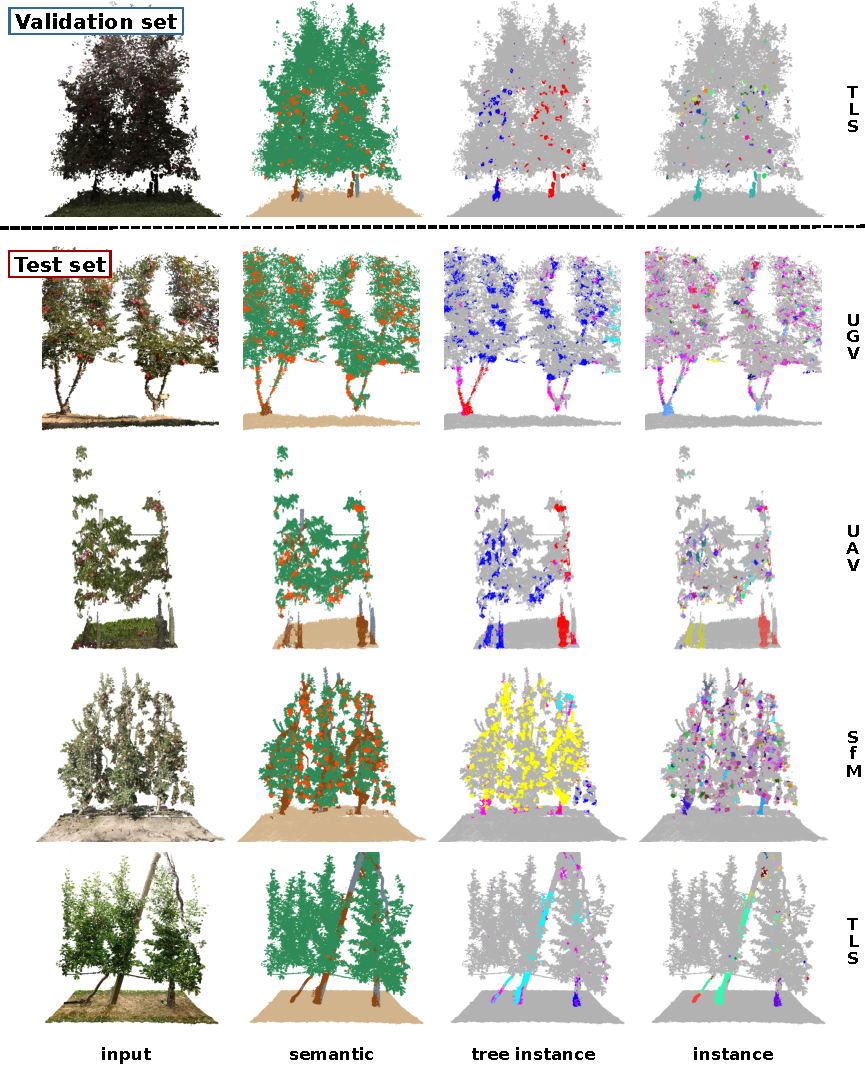
\includegraphics[width=.99\linewidth]{pics/qualitative.pdf}
  \caption{我们层次化全景分割方法的定性结果。第一行展示验证集结果,其他行展示测试集结果。我们报告了输入点云及其三种分割预测,每种传感器一个结果。在语义预测中,不同颜色表示不同类别。在实例预测中,不同颜色表示不同实例。}
  \label{fig:quali}
\end{figure*}

\subsection{消融研究} \label{sec:ablations}
在消融研究中,我们旨在验证我们的声明,即所提出的跳跃连接方案允许CNN利用分割任务之间的底层层次关系,从而获得更好的分割性能。我们在验证集上进行这个实验。我们与其他跳跃连接方案进行了比较,并在表~\tabref{tab:ablation}中报告了结果。最简单的方法不使用跳跃连接(在表~\tabref{tab:ablation}中表示为A),这导致性能不佳。这是预期的,因为解码器从早期阶段的特征中没有获得任何高级信息,这会损害梯度流。第二种方法仅使用从解码器到解码器的跳跃连接,排除来自编码器的贡献(在表~\tabref{tab:ablation}中表示为B)。这种方法尽管通过基于解码器的跳跃连接利用了任务之间的层次结构,但不能产生良好的性能。第三种方法是标准的UNet式跳跃连接,从编码器到所有解码器(在表~\tabref{tab:ablation}中表示为C)。在这种情况下,所有解码器从编码器获得相同的信息。这被证明比仅解码器跳跃连接更有效。这可能是因为恢复高级信息很重要,而使用仅解码器跳跃连接无助于梯度传播。因此,我们的方法使用来自编码器和从解码器到解码器的跳跃连接(在表~\tabref{tab:ablation}中表示为D),性能优于所有其他方法,因为一方面它受益于来自编码器的高级特征,另一方面它利用了分割任务之间的底层层次结构。有趣的是,它也在语义分割上提供了更好的结果,尽管语义解码器的跳跃连接方案没有差异,因为层次结构仅影响实例解码器。这表明来自实例解码器的信息通过反向传播间接影响编码器和语义解码器对语义分割性能有益。

\begin{table}[t]
  \caption{验证集上的消融研究。不同跳跃连接方案的比较。}
  \centering

  \begin{tabular}{cccccc}
    \toprule
    & \textbf{跳跃连接}            & \textbf{mIoU}    & \textbf{PQ}    & \textbf{PQ$_\textrm{T}$} & \textbf{mPQ}        \\
    \midrule
    A & 无 & 55.8 & 42.8 & 47.7 & 45.3\\    
    B & 解码器 & 64.4 & 53.4 & 51.3 & 52.4 \\    
    C & 编码器 & 69.8 & 58.8 & 50.9 & 54.9 \\    
    \midrule
    D & 编码器+解码器 & \textbf{70.9} & \textbf{60.8} & \textbf{52.1} & \textbf{56.5} \\    
    \bottomrule
  \end{tabular}
  \label{tab:ablation}
  \vspace{-1em}
\end{table}
\section{结论}
\label{sec:conclusion}

在本文中,我们提出了一种新的点云数据层次化3D全景分割方法。通过新颖的跳跃连接方案,我们的方法利用不同分割任务之间的底层层次结构,能够同时产生语义分割、树木实例分割(其中一棵树定义为一个树干和属于它的所有苹果)以及标准实例分割。由于我们架构中提出的跳跃连接方案,我们的方法取得了最先进的结果,超越或可与现有的任务特定基线相媲美,尽管它们一次只能处理一个实例分割任务。此外,我们引入了一个名为HOPS的新点云数据集,来自真实苹果园,标注用于层次化全景分割。我们的数据集包括两年内使用不同传感器录制的数据。在我们的实验评估中,我们支持了本文中提出的所有声明,并表明我们提出的数据集具有挑战性。

\addtolength{\textheight}{-.5cm} 

%%%%%%%%%%%%%%%%%%%%%%%%%%%%%%%%%%%%%%%%%%%%%%%%%%%%%%%%%%%%%%%%%%%%%%%%%%%%%%%%
%% Future work: Use only if applicable -- but if so, use the following
%% sentence to start:
% Despite these encouraging results, there is further space for improvements. 
%% In general, I avoid explaining future work in 6-8 page conference papers...


%%%%%%%%%%%%%%%%%%%%%%%%%%%%%%%%%%%%%%%%%%%%%%%%%%%%%%%%%%%%%%%%%%%%%%%%%%%%%%%%
% Only if applicable
%\section*{Acknowledgments}
%We thank XXX for fruitful discussions and for \dots
% \clearpage
\bibliographystyle{plain_abbrv}


% All new citations should go to new.bib. The file glorified.bib should go
% be the one from the ipb server. After paper or related work has been
% written merge the entries from new.bib to glorified.bib ON THE SERVER,
% replace the glorified.bib in this repository and empty the new.bib
\bibliography{glorified,new}

% \IfFileExists{./certificate/certificate.tex}{
% \subfile{./certificate/certificate.tex}
% }{}
\end{document}


%%%%%%%%%%%%%%%%%%%%%%%%%%%%%%%%%%%%%%%%%%%%%%%%%%%%%%%%%%%%%%%%%%%%%%%%%%%%%%%%
%% NOTES ON PAPER WRITING
%
% Rename the paper.tex file into your paper name. Use the BibTeX key policy (see below)
%
% I recommend using grammarly (www.grammarly.com) as a first check 
%
% Use a Spell Checker with US English as spelling language
%
% Use Academic Writing Check: https://github.com/devd/Academic-Writing-Check
%
% Use GIT for version control. Use our gitlab sever!
%
% Make sure your Makefile is working correctly and compiles the documents
%
% All images go to the subfolder pics and reviews into the reviews folder
%
% Make sure the source files for images are in the pics folder as well (unless they are huge)
%
%%%%%%%%%%%%%%%%%%%%%%%%%%%%%%%%%%%%%%%%%%%%%%%%%%%%%%%%%%%%%%%%%%%%%%%%%%%%%%%%


%%%%%%%%%%%%%%%%%%%%%%%%%%%%%%%%%%%%%%%%%%%%%%%%%%%%%%%%%%%%%%%%%%%%%%%%%%%%%%%%
%% NOTES ON BIB ENTRIES
%
% Bibtex Key Policy
%
%    All in lower case
%    Use the key structure: <lastnamefirstauthor><4 digit year><conference/journal><extra>
%    Use <extra>:
%        only to disambiguate: - first chars of the first 4 words f the title
%    Examples: stachniss2008icra, stachniss2008icraws, stachniss2008icra-adhc
%    Use the BibTeX key also at the filename for the paper, e.g., stachniss2008icra.pdf
%
% Bibtex Entries
%
%    Use strings for conferences and journal name in order to keep obtain consistent entries
%    Use the identical abbreviations for conference name, e.g., “Proc. of the IEEE Int. Conf. on Robotics and Automation (ICRA)”
%    Avoid adding the location in addition to the city or street of the conference.
%    Use doi for the official document on the publisher webpage.
%    Abbreviate the first name of the authors, e.g., C. Stachniss instead of Cyrill Stachniss
%    In case of a first name and a middle name, use no space between them, e.g., C.J. Stachniss
%%%%%%%%%%%%%%%%%%%%%%%%%%%%%%%%%%%%%%%%%%%%%%%%%%%%%%%%%%%%%%%%%%%%%%%%%%%%%%%%


